\documentclass[]{article}
\usepackage{caption}
\usepackage{subcaption}
\usepackage{graphicx}
\usepackage{float}
\usepackage{url}
\usepackage{amsmath}
\usepackage{amssymb}
\usepackage{tocloft}
\usepackage{wasysym}
\usepackage[shortlabels]{enumitem}
\usepackage[hidelinks]{hyperref}
\usepackage[toc,acronym,nonumberlist]{glossaries}
\setacronymstyle{long-short}
\usepackage{glossaries-extra}
\usepackage[table]{xcolor}

\graphicspath{{figs/}} 
\setlength{\cftsubsecindent}{0em}
\setlength{\cftsecnumwidth}{3em}
\setlength{\cftsubsecnumwidth}{3em}
\newcommand\numberthis{\addtocounter{equation}{1}\tag{\theequation}}

%opening
\title{
	Origins of Life Course\\
	Peer Review Assignment
}

\makeglossaries
\loadglsentries{glossary-entries}

\begin{document}

\maketitle

\tableofcontents
\listoffigures

\section{Early systems chemistry}

Figure \ref{fig:damer} shows an early protocell cycle. Identify the following parts that are
required for a biological life cycle within the figure:
\begin{table}[H]
	\caption{Early systems chemistry}	{\rowcolors{1}{green!80!yellow!50}{green!70!yellow!40}
	\begin{tabular}{|c|p{3cm}|p{8cm}|}\hline
	a&	What is the individual? &The stabilized protocell is an individual.\\
	b&	Where in the cycle are metabolic processes occurring? &Just after the head of the arrow labelled labelled "influx of solutes", during the Gel phase.\\
	c&	How does selection occur?&If protocells don't complete the anhydrous phase, they will be eliminated. \\
	d&	Is there reproduction? Why or why not? &Yes. Protocells are instantiated at end of anhydrous phase.\\
	e&	What is one energetic input found in this system?&Evaporation, which drives dehydration\cite{damer2016field}\\\hline
	\end{tabular}}
\end{table}

\begin{figure}[H]
	\caption[Early protocell cycle]{Early protocell cycle after \cite{damer2016field}}\label{fig:damer}
	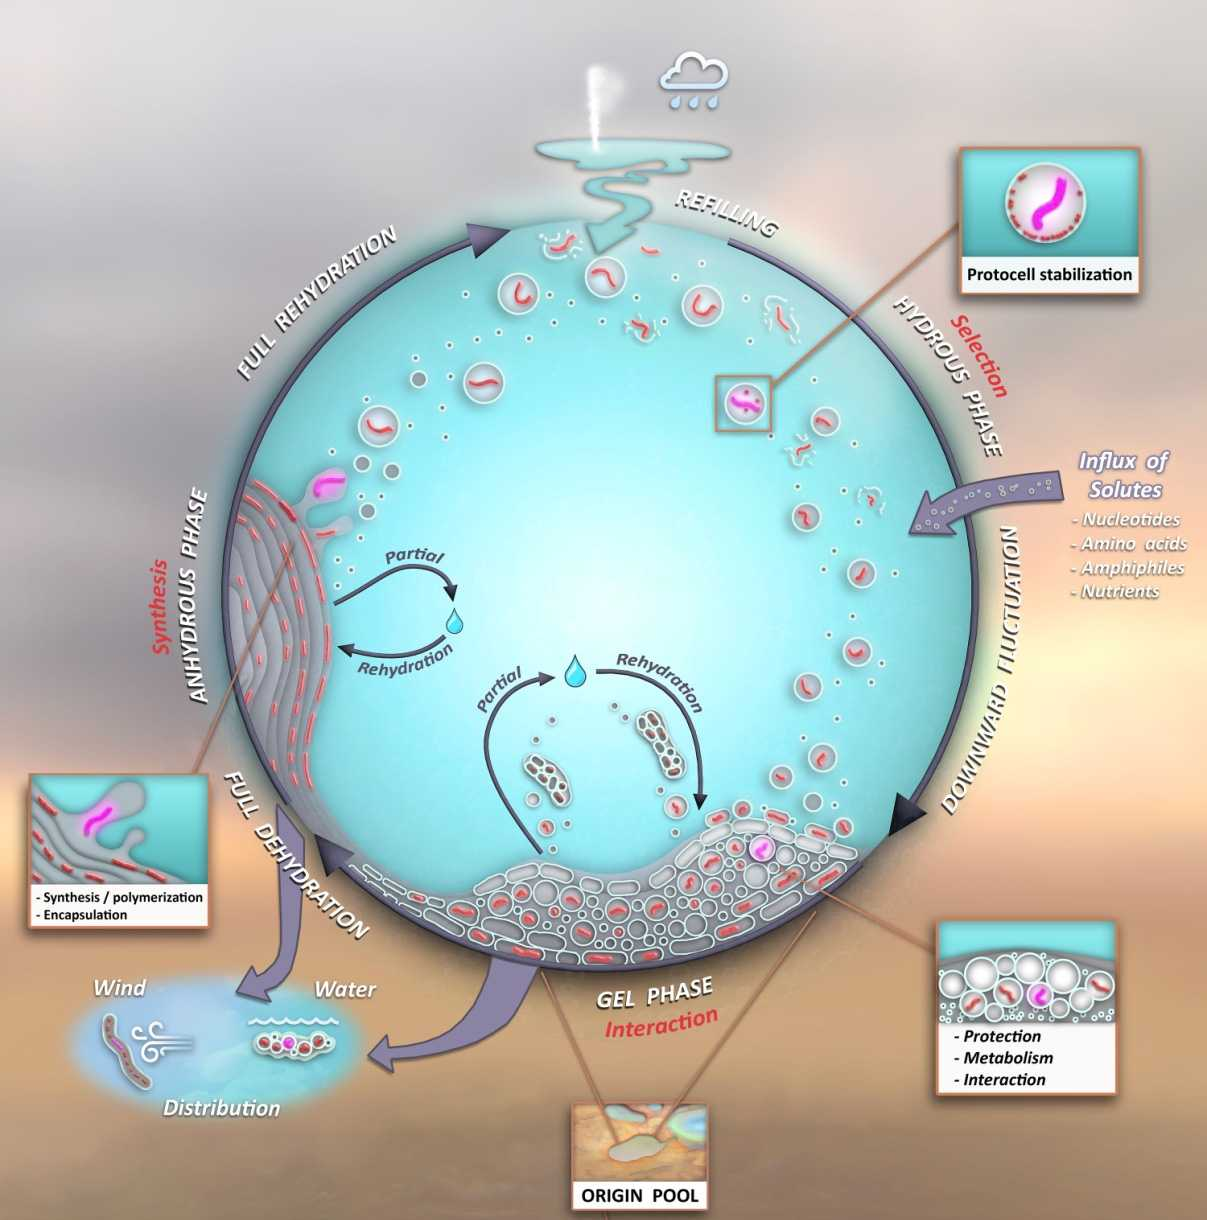
\includegraphics[width=\textwidth]{WarmLittlePond}
\end{figure}
\section{Time machine}

\begin{table}[H]
	\caption{My recommendations for Time Machine}
	{\rowcolors{1}{green!80!yellow!50}{green!70!yellow!40}
	\begin{tabular}{|c|p{3cm}|p{8cm}| } \hline
		a&What time... would you recommend they visit? &I'd be very interested in a time between 3.8 Gya and 3.5 Gya, as an intriguing but controversial case has been made for the existence of life \cite{mojzsis1996evidence,nutman2016rapid} in the Isua Greenstone belt \cite{enwiki:1095301862}--Figure \ref{fig:nuuk}. Mojzsis\cite{mojzsis1996evidence} pointed out that microfossils from 3.5 Gya were already complex, implying that there had already been considerable evolution, so a date close to 3.8 Gya would be good.\\
		b& What type of information would you want from the early Earth conditions at that
		time?& I'd like to know the atmospheric composition (especially $CO_2$, $NH_3$, and $CH_4$ ), and the the temperatures sampled during the time of the visit (which, I tryust, would not be less than one day).\\
		c& Is there a specific location/latitude you would recommend, or environment to sample		from? &Not really: everything is likely to have moved because of plate tectonics. I expect that life would have been widespread by 3.8 Gya.\\
		d& What criteria would you use to tell if the sample was “alive” or once was alive? &Since we are likely to be post-LUCA, I'd look for RNA/DNA itself.\\\hline
	\end{tabular}}
\end{table}
\begin{figure}[H]
	\caption{Nuuk region after \cite{enwiki:1095301862}}\label{fig:nuuk}
	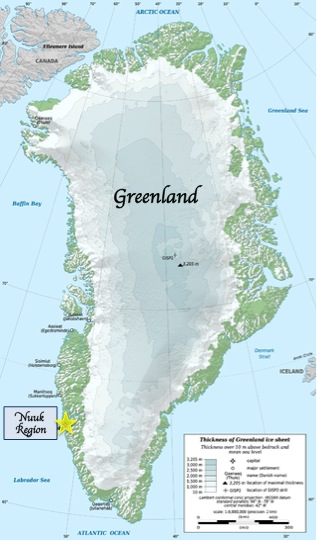
\includegraphics[width=\textwidth]{Nuuk_Location}
\end{figure}
\section{Phylogenetic tree building}
Phylogenetic tree building \cite{altschul1990basic}

\subsection{Phylogenic tree based on a single sequence}

Figure \ref{fig:Phylo1} was generated by \gls{gls:BLAST}, using 50S ribosomal protein L5 and the organisms listed in Table \ref{tab:organisms}. I chose the protein more or less arbitrarily, and then found organisms that were in the NCBI database and expressed the selected protein. I wanted representatives of all 3 super-kingdoms, archaea, bacteria, and eukaryotes.

\begin{table}[H]
	\caption{Organisms, using 50S ribosomal protein L5.}\label{tab:organisms}
	\centering
	\begin{tabular}{|l |r | p{5cm} |}
		\hline
		\textbf{Organism} & \textbf{GI} & \textbf{Remarks}\\ \hline
		Arabidopsis lyrata subsp. lyrata &297318733 & Eukaryote,  kingdom Plantae \\ \hline
		Arc I group archaeon ADurb1013\_Bin02101&1004829435&Archaeon\\ \hline
		Wolbachia endosymbiont of Drosophila melanogaster  &42410257 &Bacterium \\ \hline
		Drosophila silvestris&217426024&Eukaryote, kingdom Animalia\\\hline
		Escherichia coli &553605257 & Bacterium\\ \hline
		Pseudomonas aeruginosa &354823940 & Bacterium\\ \hline
		Shigella sonnei &903021862 &Bacterium \\ \hline
		Pyrococcus furiosus &499322460 &Archaeon \\ \hline
		Homo sapiens & 119593493&Eukaryote, kingdom Animalia  \\ \hline
		Entamoeba histolytica  &449706951&Eukaryote, phylum Amoebozoa\\ \hline
		Aigarchaeota archaeon NZ13\_MG1&1378806004&Archaeon\\ \hline
	\end{tabular}
\end{table}

\begin{figure}[H]
	\caption{Phylogenic tree based on 50S ribosomal protein L5.  Note that only one eukaryote appears, \textit{Arabidopsis lyrata}.}\label{fig:Phylo1}
	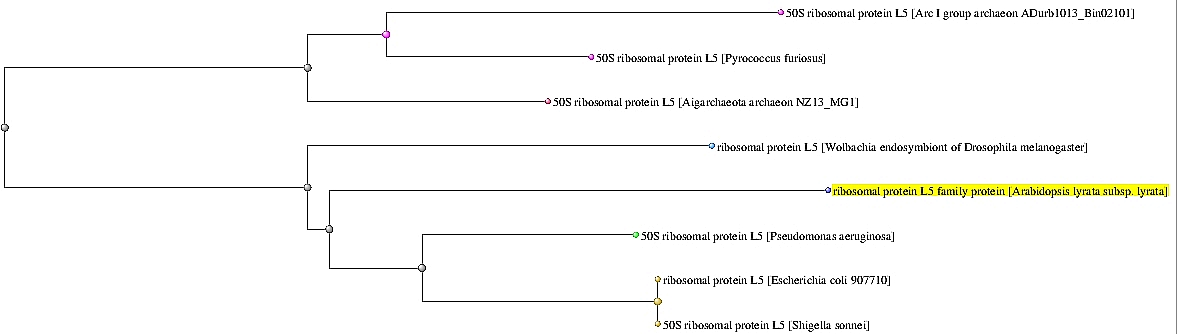
\includegraphics[width=\textwidth]{Phylo1}
\end{figure}

Note that BLAST has dropped all Eukaryotes  from the tree, except for  \textit{Arabidopsis lyrata}. I discuss this in Section \ref{sect:compare}.

\subsection{Generate a phylogenic tree based on the known taxonomy}

Figure \ref{fig:Phylo2} was generated using \cite{biobyte2019phylot}. Since the website restricted me to 9 species or fewer, I dropped two eukaryotes that were present in Table \ref{tab:organisms} but absent from Figure \ref{fig:Phylo1}.

\begin{figure}[H]
	\caption{Phylogenic tree based on the known taxonomy}\label{fig:Phylo2}
	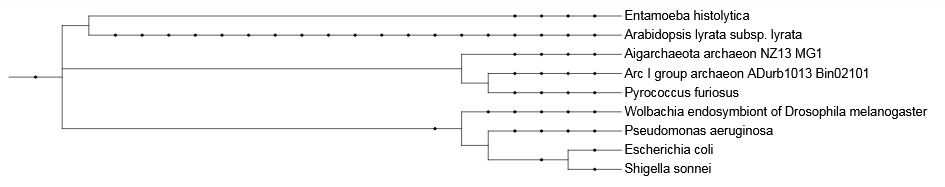
\includegraphics[width=\textwidth]{Phylo2}
\end{figure}

\subsection{Compare protein and taxonomic trees}\label{sect:compare}

\begin{enumerate}
	\item The most obvious difference between Figures \ref{fig:Phylo1} and  \ref{fig:Phylo2} is the number of nodes: neither \textit{Homo sapiens} nor \textit{Entamoeba histolytica} appear in Figure \ref{fig:Phylo1}. Since these are Eukaryotes, I assume that they were too distant from the other sequences, so BLAST dropped them from the tree. If this is the case, why is the eukaryote \textit{Arabidopsis lyrata} in the tree, and why does it appear linked to bacteria?
	\item Initially I conjectured that \textit{A. lyrata} is present because it was entered as the Query Sequence--Figure \ref{fig:BLAST1}--and the other species were entered as Subject Sequences: the others were therefore judged against \textit{A. lyrata}. However, it appears that the conjecture is incorrect, and I have observed a well-known phenomenon\footnote{This may explain why the Test suggested A. lyrata}.
	
	\begin{enumerate}
		\item  ''A 2002 study of ...\textit{A. thaiana} suggested that an unexpectedly large fraction of its genes...are derived from the cyanobacterial progenitor of the plastid\cite{lane2008eukaryotic}''
		\item ''Previous estimates have suggested that between 800 and perhaps as many as 2,000 genes in the Arabidopsis genome might come from cyanobacteria,...''.\cite{martin2002evolutionary}
	\end{enumerate} 
	\item Bacteria and archaea are generally organized similarly in  Figures \ref{fig:Phylo1} and  \ref{fig:Phylo2}.
	\item As an experiment I reran BLAST, but used \textit{Entamoeba histolytica } as the Query Sequence, and placed \textit{Arabidopsis lyrata} among the Subject Sequences. Figure \ref{fig:Phylo3} shows the results: three eukaryotes-- Homo, our "cousins" Drosophila, and Entamoeba--together with one Bacterium, \textit{Pseudomonas aeruginosa}. 
	\item Since Figures \ref{fig:Phylo1} and \ref{fig:Phylo3} suggest that \textit{Pseudomonas aeruginosa} is a rather sociable chap, I tried putting him in the Query Sequence, as shown im Figure \ref{fig:Phylo4}. The archaea are grouped together, as are most eukaryotes, except for \textit{Drosophila silvestris}, which is anomalous. Bacteria are oddly split between ones that are close to archaea, and others that are more remote.
\end{enumerate}

\begin{figure}[H]
	\caption{BLAST Query}\label{fig:BLAST1}
	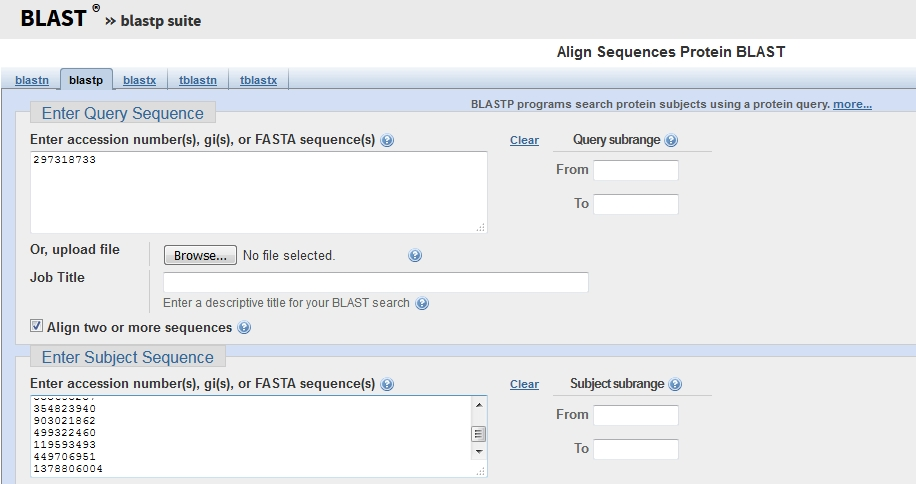
\includegraphics[width=0.8\textwidth]{BLAST1}
\end{figure}

\begin{figure}[H]
	\caption{Phylogenic tree using \textit{Entamoeba histolytica}}
	\label{fig:Phylo3}
	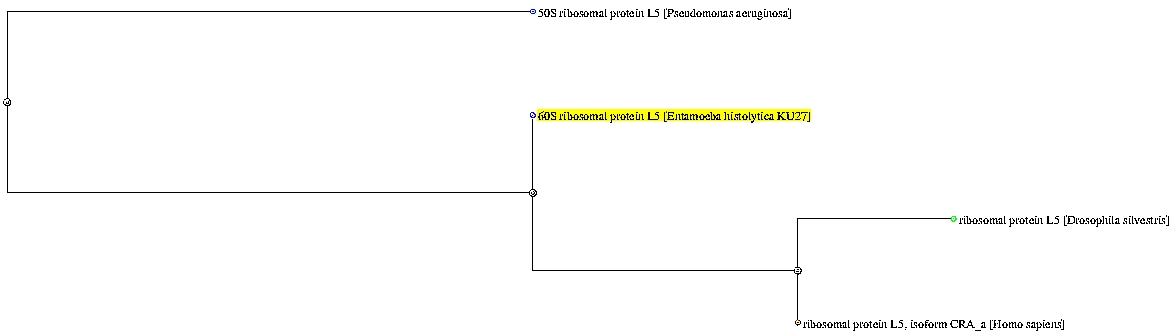
\includegraphics[width=\textwidth]{Phylo3}
\end{figure}

\begin{figure}[H]
	\caption{Phylogenic tree using \textit{Pseudomonas aeruginosa}}
	\label{fig:Phylo4}
	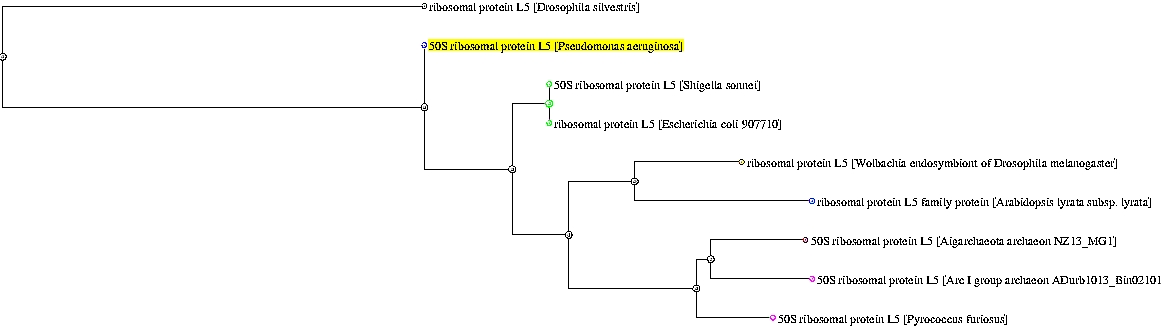
\includegraphics[width=\textwidth]{Phylo4}
\end{figure}

\subsection{Challenges building Phylogenic trees}

Section \ref{sect:compare} illustrates this.
\begin{enumerate}
	\item  In comparing the 3 super-kingdoms we are dealing with very long branches, so drift, rate heterogeneity, and long branch attraction have time to confound individual sequences. Our hope is that we can harmonize partial trees based on many sequences.
	\item Lateral Gene transfer may affect some sequences; the remedy is to base phylogenies of trees from multiple sequences.
	\item BLAST has to infer the root of the tree, by assuming that it has the least difference from the other.
	\item Because I have used representatives of the 3 super-kingdoms, there is no outgroup.
\end{enumerate}


% glossary
\printglossaries

% bibliography go here

\bibliographystyle{unsrt}
\addcontentsline{toc}{section}{Bibliography}
\bibliography{origins,wikipedia}

\end{document}
